\documentclass{article}
\usepackage{tikz}
\usepackage{amsmath}
\graphicspath{ {images/} }
\usepackage{tocloft}
\usepackage[spanish]{babel}
\usepackage{tikz}
\usepackage{tikz-3dplot}
\usepackage[style=ieee]{biblatex}
\addbibresource{referencias.bib}

\begin{document}

\title{BORRADOR INTRODUCCIÓN TFG}

\tableofcontents
\newpage

\section{Resumen}

La caracterización de antenas es una cuestión fundamental en el mundo de las telecomunicaciones sin la cual las transmisiones inalámbricas serían muy limitadas o directamente inviables. 

Debido a esto, desde que se planteó el uso de dispositivos para la transmisión de ondas electromagnéticas por aire, surgió la necesidad de poder caracterizar su comportamiento de manera fidedigna. Por lo que, durante la segunda mitad del siglo veinte, se desarrolló toda la teoría referente a la toma de medidas y la caracterización de antenas. 

No obstante, el continuo avance tecnológico termina obligando a actualizar y ampliar la forma en la que medimos antenas conforme pasa el tiempo.

Es esta necesidad de ir actualizando la forma de medir antenas a los estándares modernos lo que se pretende abordar e implementar en este documento. Con el objetivo principal de que lo estudiado y desarrollado en este documento se implemente en el Centro de Alta Tecnología y Homologación (CATECHOM) de La Escuela Politécnica de la Universidad de Alcalá. De forma que puedan tomar medidas que satisfagan los requisitos actuales a la vez que cumplen y aplican los estándares de medición establecidos por el IEEE. 

\newpage

\section{Palabras clave: TO-DO} 

Acrónimos y abreviaciones 

AUT Acrónimo de antena bajo test en inglés. 

VNA Acrónimo de analizador de redes vectoriales en inglés. 

RF Acrónimo de radiofrecuencia.

FFT Acrónimo de transformada rápida de Fourier en inglés.

IFFT Acrónimo de inversa de la transformada rápida de Fourier en inglés.

DFT Acrónimo de transformada de Fourier discreta en inglés.

\newpage

\section{Introducción }
\subsection{Sobre el documento} 

El objeto principal de este trabajo es obtener medidas del campo electromagnético radiado por una antena. De forma que, a partir de estas medidas de campo, podamos definir los parámetros característicos de la antena bajo estudio.
\\

Para ello; y dado que la idea principal es poder aplicar lo estudiado en este documento sobre medidas reales, nos hemos ceñido al estándar IEEE Std-149-2021. El cuál es el estándar vigente a fecha de escritura de este documento; y define todo lo referente a la toma de medidas de una antena.
Trabajar sobre este estándar nos fijará reglas y asunciones que conviene detallar desde el principio. Por lo que esta sección introductoria sirve a este propósito.
\\

De todo lo definido por el estándar 149-2021 nos interesan dos ideas fundamentales. La primera es que vamos a centrarnos en el estudio de antenas pasivas, lineales y recíprocas. Lo que implica que podemos medir sus propiedades independientemente de si durante el estudio la establecemos como transmisor o receptor.
\\

No obstante, es importante recalcar que el propio estándar afirma que gran parte de las prácticas pueden adaptarse al caso de medir sistemas que contengan elementos activos, no lineales o no recíprocos. Por lo que, pese a que este documento ignora este tipo de sistemas, lo descrito en él podría aplicarse a dichos casos particulares.
\\
El segundo punto clave a tener en cuenta es que el estándar; y por extensión este documento, prioriza la obtención del patrón de radiación de la antena bajo estudio. Esto se debe a que es una propiedad fundamental de cualquier antena a partir de la cual podemos obtener características como la directividad, la ganancia o la eficiencia de radiación.
\\
\newpage
\subsection{Sobre las instalaciones de medida}

La base principal para poder efectuar medidas sobre una antena es disponer de una instalación que cumpla una serie de requisitos muy concretos. Existiendo varias posibilidades válidas que satisfacen estas especificaciones. 
Esto supone que el uso de una instalación concreta determina el marco de trabajo primando una técnica de medida sobre las demás. Motivo por el cual conviene mencionar las opciones más relevantes y centrarnos en una de ellas. 
\\

Adelantándonos un poco a los contenidos, debemos tener en mente que la idea principal que permite caracterizar el comportamiento de una antena es generar una onda electromagnética plana y uniforme que incida sobre ella. 
\\

No obstante, en la práctica no podemos disponer de una onda plana y uniforme perfecta. Por lo que el objetivo principal a la hora de construir un espacio sobre el que tomar medidas es poder generar una onda lo más parecida a una onda plana uniforme. 
Bajo esta premisa fundamental, se idearon tres tipos básicos de instalaciones que permiten aproximarse al máximo a este tipo de ondas. 

\begin{itemize}
    \item \textbf{Las instalaciones de espacio libre} se diseñaron de forma que todos los efectos ajenos al entorno son suprimidos o llevados a niveles aceptables. Es decir, buscan simular lo mejor posible el vacío y usarlo como medio de transmisión. 
    \item \textbf{Las instalaciones de reflexión en tierra} pretenden beneficiarse del uso de las reflexiones sufridas por la onda de forma controlada. De forma que, a partir de la contribución de ondas reflejadas, se genera otra onda plana. Permitiendo incluso generar combinaciones de ondas planas. 
    \item \textbf{Las instalaciones de campo cercano} se idearon para poder simular una onda plana uniforme. Para lo cual se hace uso de ciertas transformaciones matemáticas efectuadas sobre las muestras tomadas durante la medición. 
\end{itemize}
De entre todos los tipos de instalaciones existentes, este documento únicamente se va a centrar en las instalaciones de espacio libre. Dado que es el tipo de instalación más común y es sobre el que vamos a trabajar.\\
Dicho esto, las instalaciones de espacio libre tienen tres subtipos de instalación principales. Las instalaciones de tipo elevada, compacta y anecoicas. De entre ellas; pondremos el foco en el tipo de instalación de que disponemos para tomar medidas. Que es la cámara anecoica. 

\newpage

\section{Análisis de las cámaras anecoicas}

Las cámaras anecoicas son instalaciones que se caracterizan por eliminar cualquier tipo de eco generado por una onda en su interior. Lo que hace que sean un entorno de medidas controlado y seguro. Dado que tenemos garantía absoluta de que las medidas realizadas en su interior no estarán contaminadas por interferencias electromagnéticas.

La motivación principal que impulsó la creación de estas cámaras es precisamente disponer de un entorno de medida aislado y perfectamente controlado. Dado que en un entorno abierto, las medidas pueden variar por factores como la climatología, la presencia de superficies reflectantes u otros factores similares que contaminarían las medidas de la antena bajo estudio. 

Es por esto que el uso de la cámara anecoica se estableció como una alternativa superior. No solo por poder controlar las condiciones climatológicas, sino por su fiabilidad en las medidas y la facilidad con la que puede variarse la frecuencia de trabajo. Permitiendo poder caracterizar el comportamiento de una antena en un rango amplio de frecuencias de forma cómoda.\\
Todo esto hace que sea un tipo de instalación ideal para la medida de antenas en las que el patrón y ubicación de la fuente sean factores clave. 

\subsection{Límites de las cámaras anecoicas}

Para poder trabajar adecuadamente con una cámara anecoica, necesitamos conocer previamente los límites de este tipo de instalaciones. Ya que, a nivel físico, existen dos factores fundamentales que restringen el uso de una cámara anecoica. Los cuales vienen impuestos por construcción y están relacionados con la capacidad de absorción de la cámara y las dimensiones de la misma. 

\subsubsection{Límite del absorbente de radio frecuencia }

Como hemos comentado, la eliminación del eco de las cámaras anecoicas nos permite controlar el entorno de medida eliminando las difracciones que puede sufrir la onda plana. Pero no hemos comentado aún nada del elemento clave que nos permite asegurar esto. El absorbente de RF. \\

El absorbente es un elemento fundamental de las cámaras anecoicas, pero que cobra una importancia mayor en nuestro caso en particular. Ya que la cámara anecoica de que disponemos es del tipo rectangular. Que es el tipo de cámara más sensible al tipo de absorbente por la forma en que incide la onda sobre él. \\

Para que el absorbente cumpla con su propósito de forma correcta, debemos asegurar que la impedancia presente en el espacio libre y la impedancia del propio material absorbente coincidan. Por lo que es habitual las cámaras tengan las paredes internas recubiertas con absorbente de RF en forma piramidal. Ya que gracias a esta estructura, se logra que ambas impedancias sean idénticas. 

Sin embargo, el uso de un absorbente con forma piramidal trae un inconveniente muy a tener en cuenta. Y es que el rendimiento del absorbente se deteriora conforme aumenta el ángulo de incidencia de la onda sobre él.\\
Es por esto que es imperativo conocer el ángulo de incidencia límite a partir del cual el absorbente es incapaz de eliminar los ecos de la onda y por tanto las medidas sufren la contaminación de ondas reflejadas.\\

Este valor suele venir definido en la hoja de características del fabricante. Pero, es interesante conocer la variación del ángulo de incidencia límite y la capacidad de absorción conforme varía la longitud de onda. Para lo cual vamos a hacer uso el estándar 149-2021. Ya que en él se define una gráfica que muestra una estimación del rendimiento de un absorbente piramidal sobre el que se aplica una onda de forma oblicua. Siendo este tipo de incidencia la presente en una cámara anecoica rectangular. 

\begin{figure}
    \centering
    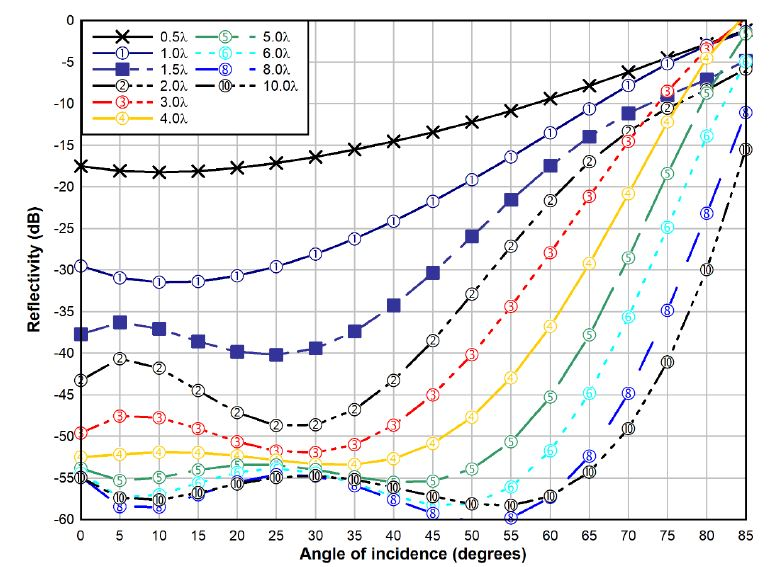
\includegraphics[scale=0.65]{Tabla-limite-angulo-incidencia}
    \caption{Gráfica con las curvas que definen la relación entre el ángulo de incidencia y la reflectividad}
    \label{Tabla-limite-angulo-incidencia}
\end{figure}

A partir de esta gráfica, podemos llegar a una conclusión relativa a la longitud necesaria que debe medir nuestro absorbente. Y es que, conque el absorbente sea más grande que una longitud de onda, en un principio podemos afirmar que el absorbente va a rendir correctamente y no vamos a sufrir ecos.

\newpage

Por lo que, si aplicamos esta idea a un ejemplo práctico para hacernos una idea de lo que supone. Significa que, si empleamos una frecuencia de 150Mhz perteneciente a la banda de la televisión, necesitamos un absorbente que mida al menos 2 m de longitud. Lo que significa que cuanto menor sea el tamaño de esta pirámide, la frecuencia mínima a partir de la cual podemos efectuar mediciones sin sufrir difracción es mayor. 

\subsubsection{Límite del tamaño de la cámara}

Al trabajar sobre una cámara anecoica rectangular, no solo debemos tener en cuenta el límite impuesto por el absorbente, sino también la longitud de la cámara. Ya que la longitud de la cámara nos va a limitar la longitud de onda mínima que podemos usar si queremos medir una antena de tamaño concreto en nuestra cámara.\\ 

Este límite se conoce como el requisito de campo lejano. El cual define una distancia a partir de la cual podemos considerar las medidas del campo como medidas del campo lejano. \\
Esta distancia es fácilmente obtenible a partir del tamaño de la antena que queremos medir y la frecuencia de trabajo usada durante la medición. Definiéndose esta distancia como: 

                            \begin{equation}
                            R =\frac{2D^2}{\lambda}
                            \end{equation}
                            
Donde D es el tamaño de apertura de nuestra antena (cuanto mide situada de perfil) y lambda es la longitud de onda en el vacío. Por lo que, asumiendo que el tamaño de la antena será de n veces lambda, podemos reescribir la ecuación como: 

                            \begin{equation}
                            R =2n^2\lambda
                            \end{equation}

Esto quiere decir, que una vez construida una cámara anecoica rectangular y conociendo cuanto mide de largo. Somos capaces de calcular cual es la longitud de onda máxima que podemos emplear para medir nuestra antena. Haciendo incluso inviable la medición de ciertas antenas en cámaras con longitud insuficiente. 

\newpage

\subsubsection{Estudio de ambos límites combinados}

Una vez presentadas y explicadas ambas limitaciones, es interesante estudiar cómo se combinan entre si. Dado que nos van a marcar la frecuencia mínima y máxima que podemos usar en una cámara. 
\\

Para ello, haremos uso de la gráfica vista en la figura \ref{Tabla-limite-angulo-incidencia}. De la cual extraemos el dato de que el absorbente piramidal de altura de $2\lambda$ debe proporcionar al menos 40dB de reflectividad. 
\\

A partir de esta reflectividad; y definiendo el ángulo de incidencia $\theta$ como el ángulo límite a partir del cual el rendimiento del absorbente decae. Podemos obtener la distancia a partir de la cual cumplimos el requisito de campo lejano.\\
Para ello, debemos aplicar trigonometría. Por lo que hemos representado el problema a resolver en la figura \ref{Geometría-del-ángulo-incidencia-absorvente} para facilitar las cosas. 

\begin{figure}[h]
    \centering
    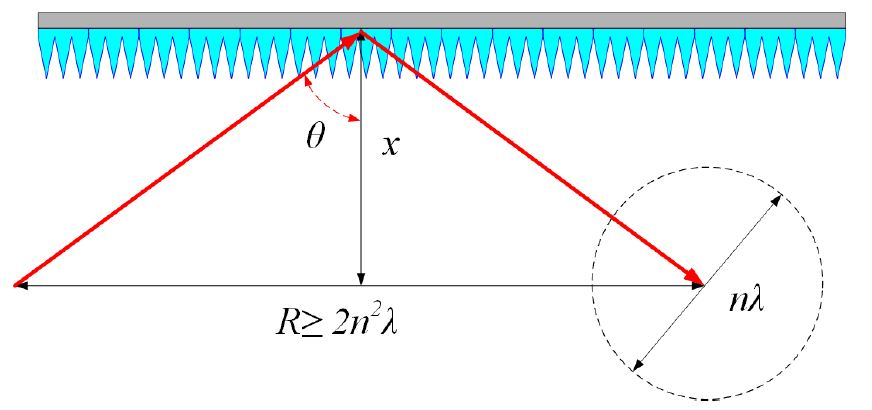
\includegraphics[scale=0.65]{Figura2-Geometria del angulo incidencia}
    \caption{Geometría del ángulo de incidencia en el absorbente de la cámara.}
    \label{Geometría-del-ángulo-incidencia-absorvente}
\end{figure}


Tras una serie de cálculos, somos capaces de obtener la siguiente expresión, que en un principio podría tomar cualquier valor: 

                        \begin{equation}
                        \tan\theta =\frac{R}{2x}
                        \end{equation}

Donde x representa la distancia desde la línea de visión hasta la superficie lateral. 

\newpage
\section{Explicación de la toma de medidas}
Tras haber dedicado una sección a comprender el tipo de instalación que vamos a utilizar y las limitaciones que implica usarla. Estamos a disposición de explicar cómo se efectúa la toma de medidas dentro de una instalación. 
\\

Y es que, en la toma de medidas, interactúan diversos sistemas de forma conjunta para poder caracterizar el comportamiento de la antena bajo test. Por lo que es interesante introducir el funcionamiento de dichos sistemas y su papel en la toma de medidas. 
\\

Dicho esto; y antes de comenzar con la sección, es interesante comentar un matiz con respecto a los contenidos que vamos a presentar. Ya que, pese a que nosotros tengamos interés únicamente en el estudio de las cámaras anecoicas rectangulares. Los sistemas aquí descritos funcionan de forma muy similar o incluso idéntica si los empleásemos en otro tipo de instalación. Por lo que las ideas y conceptos aquí descritos son en su mayoría válidos para los otros tipos de instalaciones. 

\subsection{Sistemas implicados} 

Aunque previamente hemos comentado la idea de que no todas las instalaciones valen para todos los tipos de antenas, es en este punto donde debemos destacar la importancia de esto.\\ 

Y es que, los requisitos para poder tomar medidas varían notablemente en función del tipo de antena que deseamos medir. Ya que los requisitos necesarios para caracterizar una antena pasiva de un solo puerto serán menos exigentes que los necesarios para medir una esfera de antenas de múltiples puertos usada para comunicaciones inalámbricas de alta velocidad. 
\\

Por lo que, frente a la posibilidad de tener que construir una arquitectura totalmente nueva para cada tipo de antena. Se decidió plantear un modelo lo más generalista posible. El cual encontramos definido en el estándar 149-2021 y toma la siguiente forma
\newpage

\begin{figure}[h]
    \centering
    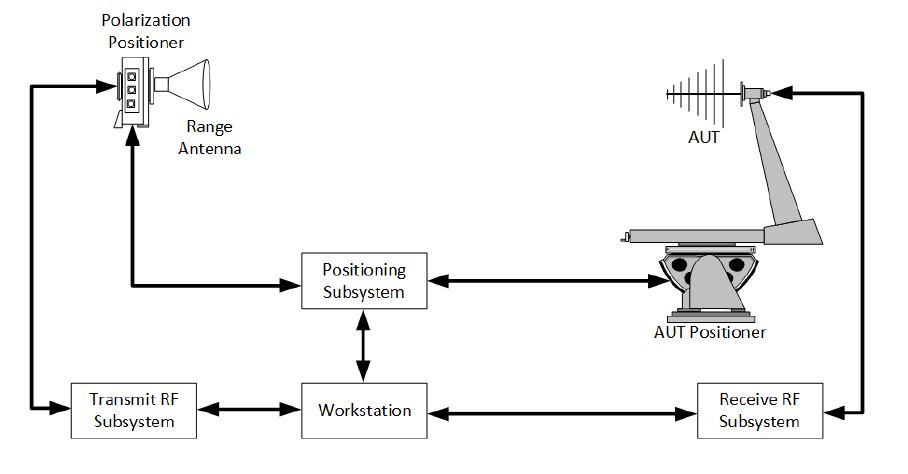
\includegraphics[scale=0.65]{Figura3-Modelo de una estacion completa de medidas}
    \caption{Modelo general de una estación de medidas.}
    \label{Modelo-general-de-una-estación-de-medidas}
\end{figure}

Este es el modelo de que disponemos y que vamos a explicar en esta sección. No sin antes hacer una aclaración con respecto a los contenidos que vamos a ver. Y es que cada uno de estos sistemas son, por si solos, objetos de estudio en sí mismos. Por lo que entrar en profundidad en su funcionamiento excede los contenidos a tratar en este documento.
\\

El objetivo de lo visto en esta sección es tener el contexto suficiente de cómo funciona y se comporta cada sistema. De manera que entendamos de dónde vienen ciertas limitaciones o porqué debemos usar ciertos sistemas de coordenadas. Vitando en la medida de lo posible detallar conceptos ajenos a nuestro campo de estudio. 

\subsubsection{Sonda} 

Si nos fijamos en la figura \ref{Modelo-general-de-una-estación-de-medidas}, nos encontramos con un elemento sobre el que no hemos hablado hasta ahora. La antena transmisora. El cual hemos ido ignorado a favor de no complicar las explicaciones anteriores.\\
Recapitulando un poco, únicamente hemos hablado de que para medir una antena requeríamos poder transmitir una onda plana uniforme; y del hecho de que en la realidad no es posible generar una onda plana perfecta. Pero no comentamos nada relacionado con como íbamos a transmitir dicha onda. Cosa que vamos a abordar en esta sección. 
\\

El uso de esta antena, denominada sonda de ahora en adelante, es necesario para poder transmitir nuestra onda plana a la AUT y así poder obtener medidas. Lo que supone que, en aras de poder conocer el comportamiento de la antena bajo test, debemos conocer a la perfección el comportamiento de nuestra sonda.
\\

Otro concepto a destacar del uso de la sonda, es la idea de que nuestro sistema de medidas pivota sobre dos antenas. Por lo que se dan diferentes configuraciones posibles en función de donde se sitúan la sonda y la AUT. Existiendo configuraciones donde están en posiciones fijas, como la ilustrada en la figura \ref{Modelo-general-de-una-estación-de-medidas}. O en las cuales se puedan intercambiar de posición. Existiendo incluso algunas instalaciones usan sistemas más pequeños cuya arquitectura combina la sonda y la AUT en una misma unidad. 
\\

No obstante, independientemente de la configuración ante la que estemos, el funcionamiento de cada sistema es idéntico. Por lo que todo lo visto a continuación es válido independientemente de dónde estén situadas las antenas. 

\subsubsection{Frecuencia de trabajo}

A excepción de algunas instalaciones especializadas en ciertos tipos de medida. Es habitual que las instalaciones de medida se diseñen para usar un rango de frecuencia lo más amplio posible que cumpla los límites aceptables de funcionamiento. Los cuales ya hemos visto cuales son y cómo calcularlos.
\\

Sin embargo, operar sobre un rango amplio de frecuencia trae consigo un problema principal. Ya que usualmente este rango de frecuencia excede el ancho de banda de trabajo de nuestra sonda. 
\\

Para solventar esto, es habitual disponer de una familia de antenas que en conjunto si permitan cubrir dicho rango de frecuencias. Lo que supone disponer de un grupo de antenas que debe tener una ganancia, ancho de haz y polarización coherentes con las medidas que queremos realizar nuestro rango.\\
Ya que no todas las antenas disponen de los mismos requisitos de línea de visión, reflexión o rangos compactos.
\\

Otro aspecto a tener en cuenta es que deseamos caracterizar la AUT en ambas polarizaciones, horizontal y vertical. Por lo que necesitamos una forma de controlar la polarización que usamos en nuestra sonda. Para esto, se suele optar por usar sondas polarizadas de forma ortogonal. Aunque también es habitual montar una sonda de polarización lineal sobre un posicionador de polarización. Lo cual permite orientar el ángulo de inclinación de la polarización.

\newpage
\subsection{Subsistema de Transmisión}

La función principal del subsistema de transmisión es generar pequeñas señales de forma controlada para estimular la antena bajo estudio. Motivo por el cual necesitamos tener muy acotados los niveles de frecuencia y potencia. 
\\

Para poder cumplir con este requisito, la selección de componentes del subsistema de transmisión depende mayoritariamente de criterios como el rango de frecuencias, el nivel de potencia a transmitir o el aislamiento. Para lo cual se suele hacer uso de una fuente que genere la señal a transmitir, un acoplador de referencia, un multiplicador de frecuencia y amplificadores. 

\subsection{Subsistema de recepción}

El propósito de este subsistema es medir la respuesta de la AUT para cada ángulo de recepción posible. Por lo que el criterio para elegir los componentes de este sistema se centra en garantizar la mayor fidelidad posible en la medición. 
\\

Centrándonos un poco en los instrumentos de medida, existen dos grupos principales: 

\begin{itemize}
    \item \textbf{Instrumentos escalares:} Son aquellos instrumentos capaces de realizar medidas en amplitud. Incluyéndose en este grupo, por ejemplo, los medidores de potencia y los analizadores de espectro. 
    \item \textbf{Instrumentos vectoriales:} Paralelo a los escalares, son aquellos instrumentos capaces de realizar mediciones de amplitud. Incluyéndose en este grupo, por ejemplo, los analizadores vectoriales de redes o los receptores de medida. 
\end{itemize}
No obstante, en la mayoría de las instalaciones modernas se mide tanto en amplitud como en fase mediante el uso de analizadores de redes vectoriales. Motivo por el que vamos a centrándonos en este tipo de instrumentación. 

\newpage

\begin{figure}[h]
    \centering
    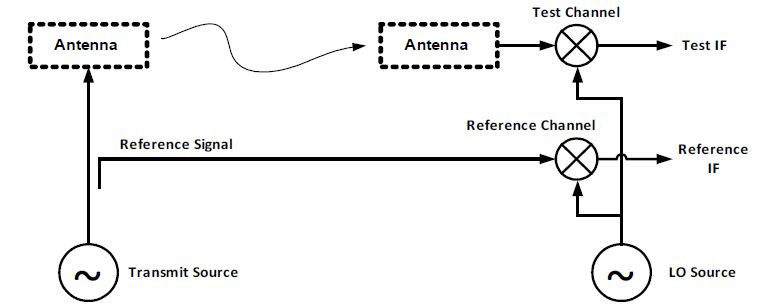
\includegraphics[scale=0.65]{Figura4-Elementos subsistema de recepcion}
    \caption{Elementos clave de un sistema de medición vectorial típico.}
    \label{Elementos-subsistema-de-recepcion}
\end{figure} 

Lo primero que podemos destacar del diagrama. Es el uso de dos canales para la medida de la fase en la AUT.\\
Uno de estos canales, el denominado canal de referencia del receptor, porta la señal de referencia generada por el subsistema de transmisión. Mientras que el otro canal, denominado canal de medición, es el que se conecta a la antena receptora y empleamos como canal de pruebas. 
\\

La respuesta en fase de la AUT se obtiene entonces midiendo la fase existente entre estos dos canales. Motivo por el cual es imperativo trabajar con la misma frecuencia en ambos canales. Para esto, se hace uso de un oscilador local común a los dos canales. Permitiendo convertir los canales a una frecuencia intermedia fija que permite digitalizar y procesar las señales. 
\\

En cuanto a la medida de amplitud. Se tiende a hacer uso de la relación de amplitud entre los dos canales. Ya que el uso de esta relación ayuda a minimizar los efectos debidos al desplazamiento de amplitud del subsistema de transmisión. 
\newpage

\subsection{Subsistema de posicionamiento} 

En el punto anterior hemos mencionado que el subsistema de recepción debe ser capaz de recibir medidas para todos los ángulos posibles. Lo cual es posible gracias a este subsistema, que es el encargado de controlar la orientación tanto de la sonda como de la AUT. 
\\

Esto supone que debe ser capaz de gestionar la carga de las antenas manteniendo a la vez la precisión de la toma de medidas. Además de introducir por primera vez la necesidad de emplear un sistema de coordenadas concreto asociado a dichas medidas. 
\\

Esto se detalla más en profundidad en las explicaciones de las transformaciones que permiten obtener el campo lejano. Pero típicamente se usa el sistema de coordenadas esféricas. Que es el que vamos a considerar aquí. 
\\

Independientemente de si la línea de visión es fijas o móvil, necesitamos disponer de dos ejes ortogonales que combinados permitan efectuar cortes en $\theta$ y $\phi$. Estos ejes se designan como el eje de rotación $\theta$ y el eje de rotación $\phi$. Los cuales están representados en la siguiente figura. 

\begin{figure}[h]
    \centering
    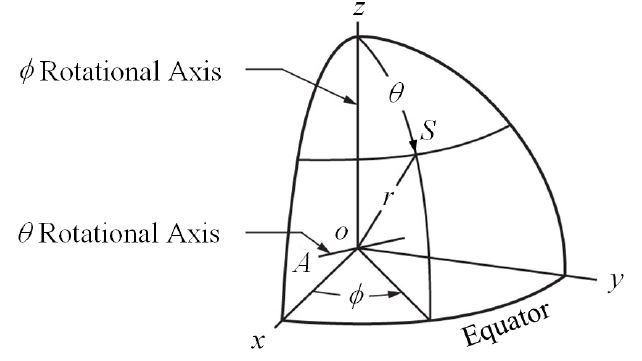
\includegraphics[scale=0.5]{Figura6-Ejes ortogonales para medir antenas}
    \caption{Ejes de rotación en un sistema esférico.}
    \label{Ejes-ortogonales-para-medir-antenas}
\end{figure} 

En nuestro caso particular, la sonda está fija y haremos pivotar la AUT de forma que podamos tomar medidas en un rango significativo de ángulos.

\newpage
\section{Transformaciones}

Hasta ahora, todo lo que hemos visto servía en última instancia como preparación para esta sección. Ya que, pese a que el objetivo principal del documento es detallar la transformación del campo medido en una cámara anecoica para poder determinar su valor en otro punto, no podíamos detallar este proceso sin antes definir el contexto sobre el cual vamos a trabajar.
\\

Por lo que, a partir de ahora, entraremos en profundidad en nuestro objeto de estudio. Siguiendo un camino natural que comienza por entender las transformaciones de puntos pertenecientes a campo cercano. Para dar el salto a las transformaciones de campo cercano a campo lejano en coordenadas planas y esféricas.
\\

Pero para esto, urge definir los conceptos de campo cercano y campo lejano. Por lo que es lo primero en lo que centraremos el foco.

\subsection{Definición del campo cercano y lejano}

Para entender de forma simple el por qué se habla de campo cercano y lejano, debemos rescatar una idea presentada anteriormente. El comportamiento de una onda conforme se aleja de la fuente que la provocó.
\\

Poniendo esta idea con un ejemplo visual, si disponemos de una superficie de agua en reposo y sobre ella dejamos caer una gota de agua, se generará una onda de forma esférica que se propaga en todas direcciones.
\\
Dicha onda irá perdiendo su forma esférica a favor de una onda plana conforme se va alejando de la fuente que la ha generado.
\\

Extrapolando esta idea a una onda electromagnética, el comportamiento es el mismo. Conforme la onda se aleja de la fuente, comprobamos que su forma se parece cada vez más a una onda plana. Hasta que, llegado un punto, la similitud es tal que podemos directamente aproximar nuestra onda como una onda plana. 
\begin{figure}[h]
    \centering
    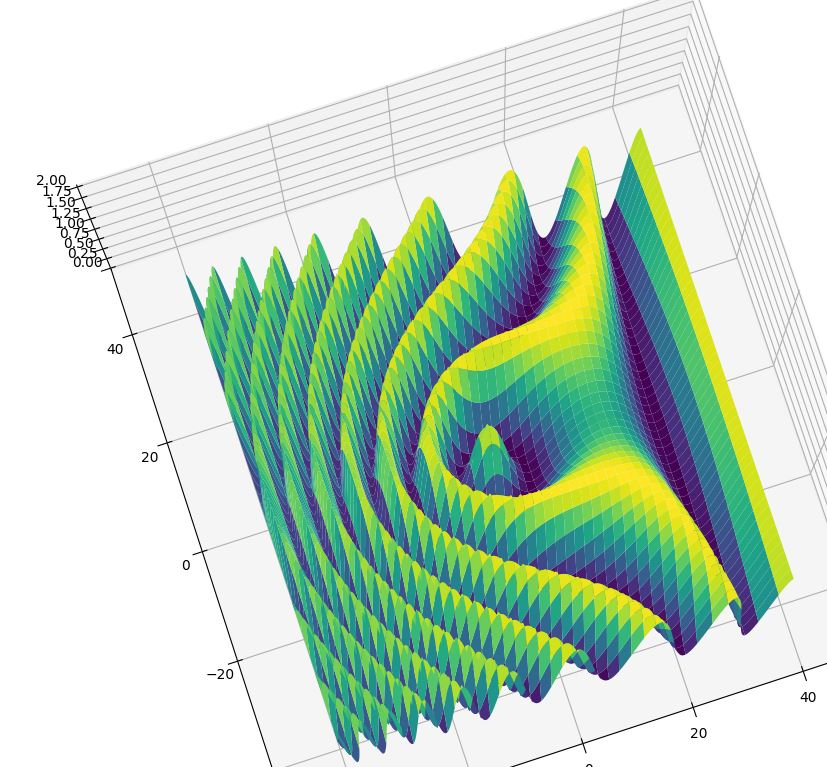
\includegraphics[scale=0.4]{Figura7-Esquema para ejemplificar el paso de onda esferica a onda plana}
    \caption{Representación visual del paso de onda esférica a onda plana}
    \label{Ejemplo-paso-onda-esferica-a-onda-plana}
\end{figure}


\newpage


Precisamente es este punto en el cual la onda puede considerarse como onda plana donde se define la frontera entre campo cercano y campo lejano. 
De manera que los valores del campo donde la onda aún no es plana pertenecen al campo cercano, mientras que aquellos valores de campo donde la onda sea próxima a una onda plana pertenecen al campo lejano. 
\\

Alejándonos de este ejemplo y pasando a términos más exactos, el campo lejano se define como la región en la que el frente de onda saliente de una antena es plano y la variación del patrón de radiación es independiente con respecto a la distancia de la propia antena.\\

Por lo tanto, para considerar una onda perteneciente al campo lejano, su componente radial debe ser despreciable en comparación con la componente transversal. Y de forma adicional, la relación entre el campo eléctrico y magnético debe ser igual a la impedancia intrínseca del medio. Debiéndose cumplir ambos requisitos en todas las direcciones angulares vistas desde la antena.\\
\newpage

Esto supone que para determinar la distancia a partir de la cual tenemos medidas pertenecientes al campo lejano, hay que verificar estas propiedades para todas las direcciones angulares. Cosa que ocurre a una distancia igual a:

\begin{equation}
                            R =\frac{2D^2}{\lambda}
\end{equation}

Donde D es la dimensión máxima de la antena y $\lambda$ es la longitud de onda de operación.\\

Si recordamos, esta fórmula ya la habíamos presentado al detallar las limitaciones presentes al usar una cámara anecoica. Lo que sirve ilustra que, en realidad, todo el rato hemos tratado con la idea de campo lejano y campo cercano.
\newpage

\subsection{Transformación entre puntos del campo cercano}

Lo primero que debemos abordar y que nos dará una base sólida para las siguientes secciones, es la transformación de un punto perteneciente a un plano $Z_1$ del campo cercano a otro plano $Z_2$ que también pertenece al campo cercano.

% Representaci ́on de los planos Z1 y Z2 en perspectiva isometrica
\tdplotsetmaincoords{70}{125} % Establecer la perspectiva
\begin{figure}[htbp]
  \centering
  \begin{tikzpicture}[tdplot_main_coords,scale=2]
    % Plano Z1 en azul
    \fill[blue!20] (0,0,0) -- (2,0,0) -- (2,2,0) -- (0,2,0) -- cycle;
    \draw[blue] (0,0,0) -- (2,0,0) -- (2,2,0) -- (0,2,0) -- cycle;
    \node[blue] at (1,1,0) {\( Z_1 \)};
    % Plano Z2 en rojo
    \fill[red!20] (0,0,1) -- (2,0,1) -- (2,2,1) -- (0,2,1) -- cycle;
    \draw[red] (0,0,1) -- (2,0,1) -- (2,2,1) -- (0,2,1) -- cycle;
    \node[red] at (1,1,1) {\( Z_2 \)};
    % Ejes
    \draw[thick,->] (0,0,0) -- (2.5,0,0) node[anchor=north east]{\( x \)};
    \draw[thick,->] (0,0,0) -- (0,2.5,0) node[anchor=north west]{\( y \)};
    \draw[thick,->] (0,0,0) -- (0,0,1.5) node[anchor=south]{\( z \)};
  \end{tikzpicture}
  \caption{Representación de los planos \( Z_1 \) y \( Z_2 \) en perspectiva isométrica.}
  \label{fig:planos_NF_Z1_Z2}
\end{figure}

Para ello, vamos a basarnos en el libro \textit{Antenna Analysis and Design} de Balanis \autocite{Balanis_2016}. Para lo cual debemos hacer un breve desarrollo con algunos cálculos previos que nos lleven a las ecuaciones vistas en este libro.
\\

Por lo que, de entrada, vamos definir la expresión de un campo eléctrico genérico y de frecuencia $\omega$.

\begin{equation}
\vec{\tilde{E}}(\vec{r},t)=\vec{E}(\vec{r})\,e^{j\omega t}
\label{NFtoNF: eq-Campo E generico}
\end{equation}

Una vez definido nuestro campo, vamos a calcular su ecuación de onda lineal. Para ello, debemos aplicar el operador $\nabla^{2}$ y agregar la constante $c$. La cual representa la velocidad de propagación de la onda.

\begin{equation}
\nabla^{2} \vec{\tilde{E}}(\vec{r},t)=\frac{1}{c}\frac{\partial^{2}
\vec{\tilde{E}}(\vec{r},t)}{\partial t^{2}}
\label{NFtoNF: eq-de-onde-campo-electrico}
\end{equation}

A partir de esta expresión, podemos llegar a la ecuación de Helmholtz. Tal y como vemos en \autocite{Pozar}. Donde, aunque usan una constante $c$ menos general que la nuestra, se llega de igual forma al siguiente resultado:
 
\begin{subequations}
\begin{align}
(\nabla^{2}+k^{2})\vec{E}(\vec{r})&=0\nonumber
\\
k&=\frac{\omega}{c}
\label{NFtoNF: eq-Helmholtz}
\end{align}
\end{subequations}

\newpage

Si ahora consideramos el campo $\vec{\tilde{E}}(\vec{r})$ como uno sobre el que podemos tomar medidas y que pertenece a un plano paralelo al eje $XY$ situado a una altura $z=z_{m}$, similar a los planos vistos en la figura \ref{fig:planos_NF_Z1_Z2}. Entonces la función bidimensional $\vec{E}(x,y,z=z_{m})$ se puede representar
mediante una integral de Fourier de la siguiente forma:

\begin{equation}
\vec{E}(x,y,z=z_{m})=\int_{-\infty}^{\infty}\int_{-\infty}^{\infty}\vec{\hat{E}}(k_{x},k_{y},z=z_{m})
\,e^{-j (k_{x} x+k_{y} y)} dk_{x} dk_{y}
\label{NFtoNF: eq-fourier-campo-electrico}
\end{equation}

Expresión que podemos introducir en \eqref{NFtoNF: eq-Helmholtz}, obteniendo:

\begin{multline}
\left(\nabla^{2}+k^{2}\right)\left(\int_{-\infty}^{\infty}\int_{-\infty}^{\infty}\vec{\hat{E}}(k_{x},k_{y},z)
\,e^{-j (k_{x} x+k_{y} y)} dk_{x}
dk_{y}\right)=\\
\int_{-\infty}^{\infty}\int_{-\infty}^{\infty}\left(\nabla^{2}+k^{2}\right)\left[\vec{\hat{E}}(k_{x},k_{y},z)
\,e^{-j (k_{x} x+k_{y} y)}\right] dk_{x} dk_{y}=0
\label{NFtoNF: eq-fourier-campo-electrico-introducida-en-Helmholtz}
\end{multline}

Donde hemos devuelto la generalidad a la $z$. Ya que, a efecto de los cálculos, puede tomar cualquier valor. Simplemente hasta ahora queríamos detallar la relación de esta componente con los planos de medida.
\\

Si ahora operamos el Laplaciano, obtenemos:

\begin{equation}
\int_{-\infty}^{\infty}\int_{-\infty}^{\infty}\left[\left(-k_{x}^{2}-k_{y}^{2}+k^{2}\right)+\frac{\partial^{2}}{\partial
z^{2}}\right]\left[\vec{\hat{E}}(k_{x},k_{y},z) \,e^{-j (k_{x}
x+k_{y} y)}\right] dk_{x} dk_{y}=0.
\label{NFtoNF: eq-fourier-campo-electrico-introducida-en-Helmholtz-con-laplaciano-operado}
\end{equation}

Pero como esta igualdad debe cumplirse para todos los valores de $x$ e $y$, el integrando ha de ser nulo. Lo que da como resultado:

\begin{equation}
\frac{\partial^{2}}{\partial
z^{2}}\vec{\hat{E}}(k_{x},k_{y},z)+w^{2}\vec{\hat{E}}(k_{x},k_{y},z)=0
\label{NFtoNF: resultado eq-fourier-campo-electrico-introducida-en-Helmholtz simplificada}
\end{equation}
Donde $w^{2}=k^{2}-k_{x}^{2}-k_{y}^{2}$.
\\

A partir de esta expresión, podemos definir una solución general de \eqref{NFtoNF: resultado eq-fourier-campo-electrico-introducida-en-Helmholtz simplificada} de la siguiente forma:

\begin{equation}
\vec{\hat{E}}(k_{x},k_{y},z)=\vec{\mathcal{E}^{+}}(k_{x},k_{y})\,e^{-j
w z}+\vec{\mathcal{E}^{-}}(k_{x},k_{y})\,e^{j w z}
\label{NFtoNF: solucion eq-fourier-campo-electrico-en-Helmholtz-general}
\end{equation}

Donde el valor $\vec{\mathcal{E}^{+}}(k_{x},k_{y})\,e^{-j w z}$  representa una onda propagada en el sentido positivo del eje $z$, Mientras que, como contrapartida, $\vec{\mathcal{E}^{-}}(k_{x},k_{y})\,e^{j w z}$ representa una onda propagada en dirección opuesta.\\

\newpage

Para nuestro caso, solamente consideraremos la solución que contiene la onda $\vec{\mathcal{E}^{+}}(k_{x},k_{y})\,e^{-j w z}$. Por lo que podemos reescribir la ecuación \eqref{NFtoNF: eq-fourier-campo-electrico} teniendo en cuenta esta solución. Lo que nos lleva directamente a la ecuación (12-73) del libro de \textit{Balanis}  \autocite{Balanis_2016}.

\begin{equation}
\vec{E}(x,y,z)=\int_{-\infty}^{\infty}\int_{-\infty}^{\infty}\vec{\mathcal{E}^{+}}(k_{x},k_{y})
\,e^{-j (k_{x} x+k_{y} y+w  z)} dk_{x} dk_{y}
\label{NFtoNF:eq-fourier-balanis}
\end{equation}

A partir de todo esto extraeremos en la siguiente sección los pasos de un
algoritmo que nos permitirá calcular el campo eléctrico en una
posición $z$ cualquiera. La cual no tiene por qué ser la de salida de la onda. Es decir, no tiene por qué corresponderse con el plano radiante de la antena, sino que puede
ser cualquier plano colocado delante de la misma.
\\

En otras palabras, hablamos de un algoritmo capaz de calcular el campo cercano en un plano
geométrico dado por una $z$ concreta a partir de los valores del campo medido en un plano anterior.\\
Pero, si nos damos cuenta, en todo este desarrollo no hemos tenido en cuenta si el campo es cercano o lejano.
Esto es así debido a que todo lo anterior es válido independientemente del valor de  $z$ a partir del cual consideramos que nuestro campo pasa a ser lejano. Sino que es a partir de este punto donde vamos a centrarnos estrictamente al campo cercano. Cosa que nos va a permitir aplicar ciertas simplificaciones.

\subsubsection{Algoritmo para transformar el valor del campo cercano medido en $z=z_{1}$ en el campo cercano en otro plano $z=z_{2}$}

Lo primero que debemos hacer es estimar los modos dados por la función
$\vec{\hat{E}}(k_{x},k_{y},z=z_{1})$. Para lo cual, hay que partir de la
ecuación \eqref{NFtoNF: eq-fourier-campo-electrico} e invertirla \footnote{En realidad, \eqref{NFtoNF:eq-fourier-campo-electrico-invertida} tiene la forma de
la transformada de Fourier directa de $\vec{E}(x,y,z=z_{1})$ como
función de $x$ e $y$, mientras que la ecuación \eqref{NFtoNF: eq-fourier-campo-electrico}
es formalmente la transformada inversa}. Lo que nos da la siguiente ecuación:

\begin{equation}
\vec{\hat{E}}(k_{x},k_{y},z=z_{1})=\frac{1}{(2\pi)^{2}}\int_{-\infty}^{\infty}\int_{-\infty}^{\infty}\vec{E}(x,y,z=z_{1})
\,e^{j (k_{x} x+k_{y} y)} dx dy.
\label{NFtoNF:eq-fourier-campo-electrico-invertida}
\end{equation}

Como las medidas de las que partimos no son continuas, sino que conocemos
el campo $\vec{E}(x,y,z=z_{1})$ en un conjunto de puntos
$(x,y)=(x_{n_{x}},y_{n_{y}})$ con $n_{x}=0,1,2,\ldots,N_{x}-1$ y
$n_{y}=0,1,2,\ldots,N_{y}-1$. Deberemos discretizar \eqref{NFtoNF: eq-fourier-campo-electrico} y, por tanto,  \eqref{NFtoNF:eq-fourier-campo-electrico-invertida}. Por lo que vamos a reescribirla de la siguiente forma.

\begin{equation}
\vec{\hat{E}}(k_{x},k_{y},z=z_{1})=\frac{\Delta x
\Delta y}{(2\pi)^{2}}
\sum_{n_{x}=0}^{N_{x}-1}\sum_{n_{y}=0}^{N_{y}-1}\vec{E}(x=n_{x}\Delta
x,y=n_{y} \Delta y,z=z_{1}) \,e^{j (k_{x} n_{x} \Delta x+k_{y} n_{y}
\Delta y)}
\label{NFtoNF:eq-fourier-campo-electrico-invertida-discretizada}
\end{equation}

Con esta ecuación somos capaces de estimar los modos para
cualquier valor de $k_{x}$ y $k_{y}$. Los cuales podríamos utilizar
luego para calcular  \eqref{NFtoNF: eq-fourier-campo-electrico}.\\
Por lo que parece conveniente utilizar el mayor número de valores posibles y construir
una malla de puntos $(k_{x},k_{y})$ mucho mayor que la existente en $(x,y)$. La cual ya hemos visto que tiene $N_{x}\times N_{y}$ puntos. 
\\

Sin embargo, este razonamiento presenta dos errores:
\begin{enumerate}
    \item No estamos teniendo en cuenta el teorema del muestreo.
    
    \item No nos permite vincular nuestro problema con el algoritmo de la transformada de Fourier rápida (FFT). 

\end{enumerate}

Decimos que este razonamiento presenta un error al no tener en cuenta el teorema del muestreo dado que no por
tomar más valores de $(k_{x},k_{y})$ vamos a tener una mejor descripción
de $\vec{E}(x,y,z)$. Puesto que hay un nivel de información máximo
asociado al muestreado en $(x,y)$.\\

Por este motivo; y para beneficiarnos de otras características fundamentales de este algoritmo, tenemos un especial interés en poder resolver nuestro problema con el algoritmo de la FFT. Ya que tanto la FFT como su inversa (IFFT) son algoritmos diseñados para tener en cuenta el teorema del muestreo.
\\

Llegados a este punto; y habiendo presentado las bondades del la FFT y la IFFT. Es interesante estudiar brevemente ambas expresiones. Por lo que vamos a comenzar definiendo la expresión de la FFT. 

\begin{equation}
\vec{\hat{E}}_{m_{x},m_{y}}=\frac{1}{N_{x} N_{y}}
\sum_{n_{x}=0}^{N_{x}-1}\sum_{n_{y}=0}^{N_{y}-1}
\vec{E}(x=n_{x}\Delta x,y=n_{y} \Delta y,z=z_{1}) \,e^{j 2\pi
\frac{m_{x} n_{x}}{N_{x}}}\,e^{j 2\pi \frac{m_{y} n_{y}}{N_{y}}}
\label{NFtoNF:eq-fft1}
\end{equation}

Y a continuación la expresión de la IFFT.
\begin{equation}
\vec{E}_{n_{x},n_{y}}=
\sum_{n_{x}=0}^{N_{x}-1}\sum_{n_{y}=0}^{N_{y}-1}
\vec{\hat{E}}_{m_{x},m_{y}} \,e^{-j 2\pi \frac{m_{x}
n_{x}}{N_{x}}}\,e^{-j 2\pi \frac{m_{y} n_{y}}{N_{y}}}
\label{NFtoNF:eq-ifft1}
\end{equation}

\newpage

Si compararamos  \eqref{NFtoNF:eq-fft1} con \eqref{NFtoNF:eq-ifft1}, vemos que para
poder aprovechar la herramienta que nos brinda la FFT debemos cumplir las siguientes igualdades:

\begin{subequations}
\begin{align}
k_{x}&= m_{x}\Delta k_{x}
\\
k_{y}&= m_{y}\Delta k_{y}
\\
\Delta x \Delta k_{x}&=\frac{2\pi}{N_{x}}
\\
\Delta y \Delta k_{y}&=\frac{2\pi}{N_{y}}.
\end{align}
\end{subequations}

De todas ellas, las más relevantes para nosotros son las dos últimas. Ya que son de obligado
cumplimiento si queremos poder interpretar la ecuación \eqref{NFtoNF:eq-fourier-campo-electrico-invertida-discretizada} como
una FFT. Y es que a partir de ellas podemos definir\footnote{Si nos fijamos, $\Delta x$ y $\Delta y$ están
definidos por el muestreado del campo medido en $z_1$. Pero los de $\Delta k_{x}$ y $\Delta k_{y}$ aún no estaban definidos.} los valores de $\Delta k_{x}$ y
$\Delta k_{y}$ como:

\begin{align}
\Delta k_{x}&=\frac{2\pi}{\Delta x N_{x}}
\\
\Delta k_{y}&=\frac{2\pi}{\Delta y N_{y}}
\end{align}

Teniendo esto en cuenta, podemos definir la relación entre 
$\vec{\hat{E}}_{m_{x},m_{y}}$ de la ecuación \eqref{NFtoNF:eq-fft1} y 
$\vec{\hat{E}}(k_{x},k_{y},z=z_{1})$ de la ecuación \eqref{NFtoNF:eq-fourier-campo-electrico-invertida-discretizada} como:

\begin{equation}
\vec{\hat{E}}(k_{x}=m_{x} \Delta k_{x},k_{y}=m_{y} \Delta
k_{y},z=z_{1})= \Delta x \Delta y\vec{\hat{E}}_{m_{x},m_{y}}
\end{equation}

Expresión que, a nivel computacional, usaremos para calcular los modos $\vec{\hat{E}}(k_{x}=m_{x} \Delta k_{x},k_{y}=m_{y} \Delta
k_{y},z=z_{1})$ de la siguiente forma:

\begin{equation}
\vec{\hat{E}}_{m_{x},m_{y}}=\mbox{FFT}\{\vec{E}(x=n_{x}\Delta
x,y=n_{y} \Delta y,z=z_{1})\}.
\end{equation}

Llegados a este punto, entramos en la segunda parte del proceso de transformación. Donde haremos uso de la IFFT como herramienta para poder calcular el campo en $z=z_2$. Para lo cual lo primero que debemos hacer es discretizar \eqref{NFtoNF:eq-fourier-balanis} para poder aproximarnos a \eqref{NFtoNF:eq-ifft1}.

\begin{equation}
\vec{E}(x,y,z=z_{2}) =
\\
\Delta k_{x} \Delta k_{y}
\sum_{m_{x}=0}^{N_{x}-1}\sum_{m_{y}=0}^{N_{y}-1} 
\vec{\hat{E}}(k_{x},k_{y},z=z_{2})
\,e^{-j(n_{x}m_{x}\Delta x  \Delta k_{x} + n_{y}m_{y}\Delta xy  \Delta k_{y})}
\end{equation}

Haciendo uso de la ecuación \eqref{NFtoNF: solucion eq-fourier-campo-electrico-en-Helmholtz-general} y manteniendo que $\vec{\mathcal{E}^{-}}(k_{x},k_{y})=0$. Entonces se cumple que:

\begin{equation}
\vec{\hat{E}}(k_{x},k_{y},z_{1})=\vec{\mathcal{E}^{+}}(k_{x},k_{y})\,e^{-j
w z_{1}}
\end{equation}

Expresión a partir de la cual podemos despejar $\vec{\mathcal{E}^{+}}(k_{x},k_{y})$ como:

\begin{equation}
\vec{\mathcal{E}^{+}}(k_{x},k_{y})=\vec{\hat{E}}(k_{x},k_{y},z_{1})\,e^{j
w z_{1}}
\end{equation}

Lo que finalmente nos permite calcular el campo en $z=z_2$ como:

\begin{equation}
\vec{E}(x,y,z=z_{2})=\Delta k_{x} \Delta
k_{y}\,\mbox{IFFT}\{\vec{\hat{E}}(k_{x}=m_{x}\Delta
k_{x},k_{y}=m_{y} \Delta k_{y},z=z_{2})\}.
\end{equation}

Advertencias:
\begin{enumerate}
\item Como el campo es vectorial, hay que aplicar separadamente este
algoritmo a todas las componentes.
\item Por supuesto, podemos trabajar con $\Delta x=\Delta y$
\item Los dos planos y las dos rejillas de medidas tienen que tener las mismas
dimensiones pero pueden ser subdominios de áreas mayores en las
cuales, por lo que sea, eliminamos ciertos márgenes. Eso ocurre en
el caso de trabajar con medidas simuladas sobre espacios esféricos,
donde los cortes con $z$'s dados no son iguales: nos quedamos con
los subdominios de iguales dimensiones.
\end{enumerate}

\newpage

\subsection{Transformación del campo cercano medido en un plano a valores de una superficie esférica}

Una vez comprendido el proceso que nos permite transformar medidas entre dos planos medidos en campo cercano, estamos a disposición de comprender cómo es la transformación de campo cercano en campo lejano.\\

Sin embargo, en esta ocasión no nos limitaremos a transformar las medidas de un plano a otro posterior. Sino que esta vez nuestro objetivo es poder transformar las medidas del campo cercano efectuadas sobre un plano en coordenadas cartesianas a las pertenecientes en una superficie esférica. Puesto que, como hemos detallado en secciones anteriores, la medición de antenas busca poder conocer el valor del campo en coordenadas esféricas. Ya que són las de mayor interés.
\\

Para ello, vamos a partir de la definición de un campo eléctrico cualquiera cuyos valores pertenecen al campo lejano.

\begin{equation}
\vec{E}(x,y,z)=\frac{jk_{z}}{2\pi r}\,e^{-jk_{0}r}{\vec{\mathcal{E}}}(k_{x}=k \sin\theta \cos\phi,k_{y}= k\sin\theta \sin\phi)
\label{NFtoFF:eq-campo-lejano}
\end{equation}

Donde $k_{x}$ y $ k_{y}$  contienen la información de los ángulos del sistema de referencia esférico que sirve de base para la expresión del diagrama de radiación en el campo lejano. Mientras que el valor de $k_{z}$ se corresponde con $k\cos\theta$, siendo $k$ el número de onda en el vacío.
\\

Para nuestra transformación, lo que realmente nos interesa es el valor del espectro. Es decir, la función de modos ${\vec{\mathcal{E}}}(k_{x},k_{y})$. La cual viene dada por la siguiente expresión:

\begin{equation}
{\vec{\mathcal{E}}}(k_{x},k_{y})=\int_{-\infty}^{\infty}\int_{-\infty}^{\infty}\vec{E}(x,y,z=z_{0})\,e^{-j k_{x}x}\,e^{-jk_{y}y} dx dy.
\label{NFtoFF:eq-modos-del-campo-lejano}
\end{equation}
 
A partir de esta expresión podemos extraer una característica muy importante. Y es que la extracción de las componentes modales no depende del plano $z$, sino que puede tomar cualquier valor. Lo que significa que, mientras las medidas de dicho plano pertenezcan al campo cercano, la descomposición será siempre la misma.
\\

Por otro lado, debemos tener en cuenta que en realidad solo conoceremos como es el campo  $\vec{E}(x,y,z=z_{0})$ en un conjunto discreto de puntos $(x,y) = (x_{n_{x}},y_{n_{y}})$ con  $n_{x}=0,1,2,\ldots,N_{x}-1$ y  $n_{y}=0,1,2,\ldots,N_{y}-1$. Por lo que debemos reescribir nuestra ecuación de modos paara que se ajuste a este conjunto de valores. Aprovechando la ocasión para adaptar la ecuación de forma que podamos hacer uso de la transformada discreta de Fourier. Ya que, de nuevo, vamos a hacer uso de la FFT como herramienta para poder efectuar la transformación.
\\

Con todo lo anterior en mente,  nuestra $\vec{\mathcal{E}}(k_{x},k_{y})$ pasa a tener la siguiente forma: 
\begin{align}
{\vec{\mathcal{E}}}(k_{x},k_{y})&=\frac{L_{x}L_{y}N_{x}N_{y}}{4 \pi^2 (N_{x}-1)(N_{y}-1)} \nonumber \\
&\times \sum_{n_{x}=1}^{N_{x}-1}\sum_{n_{y}=1}^{N_{y}-1} DFT(\vec{E}(x=n_{x}\Delta
x,y=n_{y}\Delta
y,z=z_{0}))\,e^{-j k_{x}n_{x} \Delta x}\,e^{-jk_{y}n_{y} \Delta y}
\label{NFtoFF:eq-fourier}
\end{align}
donde:
\begin{itemize}
    \item $N_{x}$ y $N_{y}$ son, respectivamente, el número de puntos del campo cercano en la dirección $x$ e $y$ .
    \item $L_{x}$ y $L_{y}$  es la longitud de la apertura en las dimensiones  $x$ e $y$.
\end{itemize}

Llegados a este punto, hemos obtenido la expresión de la descomposición modal. Sin embargo, debemos ajustar los valores  $k_{x}$ y $k_{y}$ para poder aplicar la DFT. Para lo cual basta con discretizar los valores de  $k_{x}$ y $k_{y}$  de la siguiente forma: 

\begin{subequations}
\begin{align}
k_{x}&= m_{x}\Delta k_{x}
\\
k_{y}&= m_{y}\Delta k_{y}
\\
\Delta x \Delta k_{x}&=\frac{2\pi}{N_{x}}
\\
\Delta y \Delta k_{y}&=\frac{2\pi}{N_{y}}.
\end{align}
\end{subequations}

Es importante destacar que hemos podido hacer este paso debido a que hay una definición implícita de $k_{x}$ y $k_{y}$ . Ya que, a partir de la teoría de la DFT  y de su valor como estimador espectral, necesitamos que la multiplicación de $\Delta x \Delta k_{x}$ sea igual a $\frac{2\pi}{N_{x}}$ para poder convertir la expresión en una sobre la cual poder hacer la DFT. 
\\

Si volvemos al contexto de nuestras medidas y del algoritmo que las convierte en valores en dicho campo lejano, nos damos cuenta que estamos trabajando precisamente con una malla regular de valores  $k_{x}\times k_{y}$. Los cuales son coordenadas cartesianas del sistema de referencia del dominio transformado. Por lo que a partir de esta malla, podemos dar una correspondencia entre los valores de $k_{x}$ y $k_{y}$ y los valores pertenecientes a una malla irregular en el dominio angular de dimensiones $\theta \times \phi$.

\newpage

Discretizando entonces los valores de $k_{x}$ y $k_{y}$ de \eqref{NFtoFF:eq-fourier} obtenemos: 

\begin{equation}
{\vec{\mathcal{E}}}_{m_{x},m_{y}}=\frac{1}{N_{x} N_{y}}
\sum_{n_{x}=0}^{N_{x}-1}\sum_{n_{y}=0}^{N_{y}-1}
\vec{E}(x=n_{x}\Delta x,y=n_{y} \Delta y,z=z_{0}) \,e^{j 2\pi
\frac{m_{x} n_{x}}{N_{x}}}\,e^{j 2\pi \frac{m_{y} n_{y}}{N_{y}}}
\label{eq-fft1}
\end{equation}

Lo que finalmente nos permite reescribir \eqref{NFtoFF:eq-campo-lejano} como a continuación. Donde hemos introduciendo el uso de los ángulos $\theta \times \phi$:

\begin{align}
\vec{E}(r,\theta,\phi)&=\frac{jk_{z}}{2\pi r}\,e^{-jk_{0}}{{\vec{\mathcal{E}}}}(k_{x}=k \sin\theta \cos\phi,k_{y}= k\sin\theta \sin\phi)\nonumber
\\
\vec{E}(r,\theta_{m},\phi_{m})&=\frac{jk_{z}}{2\pi r}\,e^{-jk_{0}}{{\vec{\mathcal{E}}}}(k_{x}=m_{x}\Delta k_{x},k_{y}= m_{y}\Delta k_{y})=\frac{jk_{z}}{2\pi r}\,e^{-jk_{0}}{{\vec{\mathcal{E}}}}_{m_{x},m_{y}}\nonumber
\\
\label{eq-fourier3}
\end{align}

El uso de esta expresión trae consigo un posible problema. Y es que los valores de los ángulos $\theta \times \phi$ pueden corresponder a valores que no formen parte de nuestra malla $k_{x}\times k_{y}$. Por lo que, para solucionar esto, debemos hacer uso de una interpolación y así obtener el valores de los ángulos pertenecientes a la malla $k_{x}\times k_{y}$.
\\

Advertencias:
\begin{enumerate}
\item Si efectuamos este cálculo sobre una antena bajo test, debemos saber que tiene una limitación ligada a cómo medimos físicamente la antena. Ya que solo será válido mientras respetemos ángulos de medidas menores a los siguientes:
\begin{equation}
\vartheta = \pm\arctan \frac{S-D}{2r_{0}}
\end{equation}
Donde "$S$" es la longitud del área de muestreo: $D$  es el diámetro de la antena bajo test; y $r_ {0}$ es la distancia de separación entre la abertura de la antena bajo test y el plano de medida.
\end{enumerate}

\newpage

\subsection{Transformación del campo lejano a partir del campo cercano medido en coordenadas esféricas}

Pese a haber explicado la obtención del campo lejano a partir de medidas realizadas sobre un plano en coordenadas cartesianas. Nuestro verdadero interés está en poder obtener el campo lejano a partir de medidas del campo cercano en coordenadas esféricas.
Ya que, de forma típica, los diagramas de radiación de campo lejano suelen representarse sobre el sistema de coordenadas esférico. \\

Estando ambos sistemas de coordenadas relacionados de la siguiente forma:


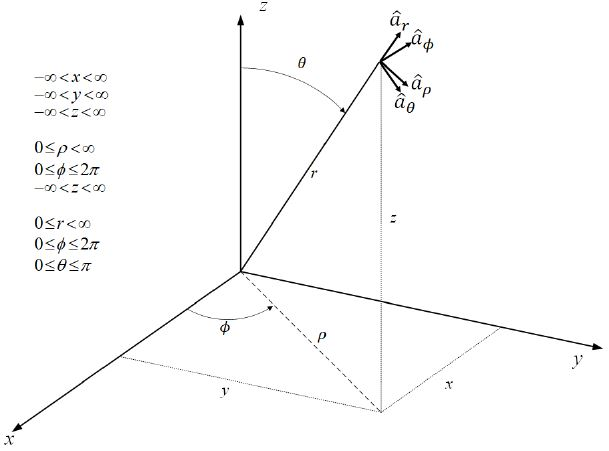
\includegraphics[scale=0.65]{relacion_esfericas_cartesianas}

\\ 

Aunque trabajar con coordenadas esféricas es más complicado, la razón principal para utilizarlas radica en que el sistema de medición de las antenas bajo prueba emplea este tipo de coordenadas.\\
Esto se debe a  que el propósito de la medición es caracterizar el comportamiento de la antena bajo estudio en todas las direcciones. Para lo cual,  la mejor forma es emplear un sistema de coordenadas esférico que tenga como origen la propia antena sobre la que deseamos obtener medidas.
\\

Una vez introducido y justificado el uso de coordenadas esféricas, es necesario enfocarnos en plantear nuestro problema de manera que podamos resolverlo utilizando este sistema de coordenadas. \\
Para ello, lo primero que debemos tener en cuenta, es que vamos a tratar con ecuaciones de ondas esféricas. Por lo que es necesario disponer de, al menos, la base fundamental de estas ecuaciones.

\subsubsection{Teoría básica de ecuaciones esféricas}

Dado que nuestro problema pertenece a un sistema de coordenadas curvilíneo,  el uso de ecuaciones diferenciales sobre nuestro campo presenta dificultades añadidas. \\
Sin embargo, podemos reducir su complejidad aprovechando una característica de estas ecuaciones. La cual nos permite tratar la resolución de ecuaciones diferenciales hechas sobre un vector (en nuestro caso, el campo eléctrico), si consideramos que podemos obtener dicho vector a partir dos vectores parciales.\\
No obstante, esta propiedad  solo puede aplicarse en caso de que los vectores parciales sean derivables a partir de una función puramente escalar que satisfaga las ecuaciones de onda vectoriales. \\

Adelantándonos un poco a lo explicado a continuación. Nosotros  siempre vamos a tratar con vectores que pueden descomponerse en vectores parciales. Cosa que vamos a demostrar en el siguiente punto.No obstante, por el momento, nos basta con saber que ciertos vectores pueden ser descompuestos en otros parciales; y que este caso particular es el que nos interesa estudiar.
\\
Dicho todo esto, la condición fundamental que permite que hagamos uso de estos vectores parciales, es que cumplan las ecuaciones de onda vectoriales. Motivo por el cual vamos a centrar nuestra atención sobre estas ecuaciones.

\subsubsection{ecuaciones de onda vectoriales}

Estas ecuaciones son, por si solas, un objeto de estudio bastante complejo.  No obstante, a nosotros solo nos interesa su uso aplicado a nuestro caso particular.
Lo cual nos va a permitir hacer una serie de simplificaciones que iremos detallando y justificando sobre la marcha.\\

De entrada, vamos a partir rescatando la idea de que vamos a hacer uso  de una cámara anecoica para realizar las medidas. Lo que significa que vamos a tener un entorno de medición con unas condiciones prácticamente iguales a las del vacío. \\
Por tanto, disponemos de un dominio cerrado (es decir,  un conjunto que incluye todos sus puntos, incluidos los puntos límite; y cuyo complemento es un conjunto abierto) con un medio de propagación isotrópico sin fuentes.\\

Este entorno en particular resulta ser el más favorable a la hora de tratar con ecuaciones de onda vectoriales. Ya que cualquiera de los vectores de campo ($E$,$B$,$D$ y $H$),  el vector potencial $A$ o  los vectores de potencia de Hertz, satisfacen una única ecuación diferencial. La cual cumplen todos ellos; y que toma la siguiente forma:
\begin{equation}
\nabla^2C - \mu\varepsilon\frac{\partial^2C}{\partial^2{t}} - \mu\sigma\frac{\partial C}{\partial{t}} = 0\
\label{eq-esfvec-general}
\end{equation}
Donde $C$ representa cualquiera de los posibles vectores citados anteriormente.\newpage
A partir de esta ecuación general, lo primero que podemos hacer es emplear la propiedad de que las ecuaciones de onda esférica son lineales. Esto nos permite simplificar la implicación del tiempo de nuestra ecuación.\\
Ya que, gracias a la linealidad, podemos reconstruir aquellos vectores que tengan una variación arbitraria con el tiempo a partir de soluciones armónicas. Permitiéndonos reescribir la ecuación sin perder con ello la generalización en nuestra expresión. \\

Es decir, podemos afirmar que nuestro vector  $C$ únicamente varía con respecto al tiempo en base al factor $e^{-jwt}$. 
Además, podemos simplificar más nuestra expresión si recordamos que el operador laplaciano ($\nabla^2$) aplicado sobre un vector cualquiera equivale a lo siguiente:
\begin{equation}
\nabla^2C =\nabla\nabla C - \nabla\times\nabla\times C + k^2C
\label{eq-nabla-sobre-vector}
\end{equation}
Con $k^2$ = $\mu\varepsilon w^2 + j\mu\sigma w$ .\\

Por lo que, aplicando todo esto, podemos reescribir  \eqref{eq-nabla-sobre-vector} de la siguiente forma:
\begin{equation}
\nabla\nabla C - \nabla \times \nabla \times C + k^2 C = 0\label{eq-esfvec-simplificada}
\end{equation}
Para poder tratar con esta ecuación, disponemos de dos alternativa: 

\begin{enumerate}
    \item Podemos optar por el camino tradicional. El cual pasa por resolver \eqref{eq-esfvec-simplificada} como un sistema de tres ecuaciones escalares.
    \item Podemos simplificar la resolución de \eqref{eq-esfvec-simplificada} resolviendo tan solo tres ecuaciones escalares independientes. Pero solo podemos considerar esta opción \textbf{si y solo si} podemos obtener $C$ a partir de sus componentes rectangulares.
\end{enumerate}

De estos dos métodos, siempre vamos a preferir el segundo. Ya que la resolución del sistema implica una alta complejidad en los cálculos. Sobretodo si la comparamos con la resolución de las tres ecuaciones independientes. \\

Volviendo a centrar la atención a nuestro problema en particular, tenemos la opción de aplicar el segundo método. Ya que siempre vamos a ser capaces de obtener el campo medido a partir de sus componentes rectangulares.\\
Lo cual se justifica dado que nuestras medidas van a cumplir siempre las propiedades de ortogonalidad.\\

Por lo que, llegados a este punto, podemos reescribir \eqref{eq-esfvec-simplificada} de la siguiente manera:
\begin{equation}
\nabla^2C_{j} + k^2C_{j} = 0
\label{eq-nabla-cuadrado-coordenada}
\end{equation}
Donde $C_{j}$ hace referencia las componentes ($x$,$y$,$z$) del vector $C$.\\
\newpage
A partir de este resultado, tendremos tantas soluciones como vectores $C$ existan. Por lo que, de ahora en adelante, vamos a considerar $\psi$ como una función escalar que es solución de \eqref{eq-nabla-cuadrado-coordenada}.\\
\begin{equation}
\nabla^2\psi + k^2\psi = 0
\label{eq-nabla-cuadrado-coordenada-con-una-soculicon-por-vector-C}
\end{equation}

De esta forma; y considerando  '$a$' como un vector unitario constante cualquiera, podemos escribir tres vectores independientes a partir de $\psi$. Los cuales son, de hecho, solución de \eqref{eq-esfvec-simplificada}:
\begin{subequations}
\begin{align}
    L&= \nabla\psi \label{eq:Lirrotacional}\\
    M&= \nabla\times a\psi\\
    N&=\frac{1}{k}\nabla\times N
\end{align}
\end{subequations}

Una vez planteadas estas tres ecuaciones, vamos a detenernos brevemente para citar algunas propiedades presentes en ellos.\\
De entrada, gracias a que '$a$' es un vector unitario, podemos reescribir $M$ de la siguiente manera:    
\begin{equation}
M= L \times a = \frac{1}{k}\nabla \times N
\label{eq-M-reescrito}
\end{equation}
Además,  para nuestra posible solución $\psi$, el vector $M$ es perpendicular a $L$. O lo que es lo mísmo, $L\cdot M=0$.\\

Al margen de a estas propiedades de $M$, por definición, las ecuaciones $L$, $M$ y $N$ presentan algunas características muy interesantes.\\
Por un lado, para $L$ se cumplen las siguientes dos propiedades:
\begin{align}
    \nabla  \times L &=0 \\
    \nabla  \cdot L  &=\nabla^2\psi = -k^2 \psi
\end{align}
Donde hemos aplicado la ecuación \eqref{eq:Lirrotacional} para obtener el carácter rotacional del vector $\vec{L}$ y convertir su divergencia en un laplaciano. \\
Con respecto a  $M$ y $N$, si rescatamos la idea de que estamos tratando vectores de campo eléctrico, significa que tanto $M$ como $N$ son capaces de crear un campo magnético.\\
Como además estamos considerando vectores pertenecientes a un medio prácticamente igual al vacío, significa que sus divergencias son nulas para cualquier punto dentro de este dominio.\\
O lo que es lo mismo,  los vectores $M$ y $N$ cumplen la condición de campo solenoidal:
\begin{align}
    \nabla\cdot M &= 0
    \label{M-cumplen-ser-campo-solenoidal}\\
    \nabla\cdot N &= 0
    \label{N-cumplen-ser-campo-solenoidal}
\end{align}
\newpage
Una vez estudiadas todas estas propiedades de los vectores $L$, $M$ y $N$. Debemos tener en cuenta que existen 3 tipos de soluciones para una ecuación diferencial, la general, la particular y la singular.\\
En nuestro caso, dado que estamos suponiendo que para cada punto existe una única solución $C$, lo que hemos estado manejando hasta ahora son, por definición, las soluciones particulares de \eqref{eq-nabla-cuadrado-coordenada-con-una-soculicon-por-vector-C}. \\
Asique, de ahora en adelante, vamos a hacer uso de la notación $\psi_{n}$ para hacer referencia a cualquiera de estas soluciones particulares de la ecuación diferencial. Existiendo entonces para cada solución  $\psi_{n}$; un conjunto de vectores $L_{n}$, $M_{n}$ y $N_{n}$.
\\

Llegados a este punto, ya tenemos todos los resultados que nos interesaban de las ecuaciones de onda vectoriales. De todo lo visto, realmente solo nos interesan los valores de   $M_{n}$ y $N_{n}$.\\
Esto se debe a que en caso de que la función dada sea solenoidal (su divergencia es nula en el dominio), su extensión se puede obtener únicamente en términos de  $M_{n}$ y $N_{n}$. 
\\

Recapitulando entonces con la idea de poder simplificar las ecuaciones de onda esférica. Hemos encontrado los vectores parciales que nos permiten representar el campo. Es decir, podemos utilizar $M$ y $N$ como vectores parciales de $E$ y $H$.\\

En resumen, si se cumple:
\begin{enumerate}
    \item Que la variación arbitraria del tiempo entra en juego únicamente como un factor armónico $e^{-jwt}$.
    \item Que estamos trabajamos con un medio donde la densidad de cargas libres es nulo en todas partes.
    \item   Que nuestro medio es isotropico.
    \item Podemos caracterizar la conductividad de nuestro medio de forma única con valor $\sigma$.

\end{enumerate}
Solo entonces podremos definir los campos $E$ y $H$ de esta forma:
\begin{equation}
E = \frac{jw\mu}{k^2}\nabla \times H\xrightarrow{}   H= \frac{1}{jw\mu}\nabla \times E
\label{campo-EyH-cumpliendo-simplificacion-con-MnyNn}
\end{equation}
Por lo que, suponiendo que el vector potencial también puede ser representado por una expansión de funciones vectoriales características. Entonces podemos escribir el valor del vector potencial como:
\begin{equation}
A = \frac{1}{w}\sum_{n}(a_{n}M_{n}+b_{n}N_{n}+c_{n}L_{n})
\label{vector-potencial-cumpliendo-simplificacion-con-MnyNn}
\end{equation}
Donde los coeficientes $a_{n}, b_{n}, c_{n}$ pueden ser obtenidos a partir de la distribución de carga del campo.

Aqui es donde entran en juego las propiedades de $L_{n}$, $M_{n}$ y $N_{n}$. Ya que gracias  a las propiedades vistas en \eqref{M-cumplen-ser-campo-solenoidal} y \eqref{N-cumplen-ser-campo-solenoidal}; a poder ignorar el vector $L_{n}$; y haciendo uso de la relación $\mu H = \nabla \times A$. Podemos escribir las ecuaciones de campo como:
\begin{align}
    E &= - \sum_{n}(a_{n}M_{n}+b_{n}N_{n})\\
    H &= - \frac{k}{jw\mu}\sum_{n}(a_{n}M_{n}+b_{n}N_{n})
\end{align}
Es decir, ya somos capaces de expresar nuestro campo eléctrico a partir de las funciones de onda esférica $M_{n}$ y$N_{n}$ y los coeficientes de onda $a_{n}$ y $b_{n}$. \\
Por lo que, podemos definir un campo eléctrico medido en coordenadas esféricas de la siguiente manera:
\begin{equation}
\vec{E}(r,\theta,\phi)=\sum_{n=-Nm}^{Nm}(a_{n}M_{n}(r,\theta,\phi)+b_{n}N_{n}(r,\theta,\phi))
\label{eq-campoE-coordenadas-esfericas}
\end{equation}
\newpage
\subsubsection{Método para la obtención del campo lejano}
Hasta ahora hemos hecho referencia a campos. Pero lo que realmente va a interesarnos a partir de ahora es el estudio de los  modos del campo eléctrico.\\
Es por esto que debemos mencionar el desuso  del subíndice  $n$ que hemos venido usando hasta ahora para representar que tratábamos con soluciones particulares de la ecuación diferencial.\\
Ya que a partir de ahora, vamos a referirnos siempre a modos, por lo que usaremos el subíndice $m$ y $n$ para ello.\\

Es por esto por lo que de ahora en adelante, en lugar de usar la ecuación del campo eléctrico definida en \eqref{eq-campoE-coordenadas-esfericas}, vamos a reescribirla para poder obtener $\vec{E}(r,\theta,\phi)$ a partir del desarrollo de sus modos:
\begin{equation}
\vec{E}(r,\theta,\phi)=\sum_{m=-M}^{M}\sum_{n=-N}^{N}\big[a_{n}M_{mn}(r,\theta,\phi)+b_{n}N_{mn}(r,\theta,\phi)\big]
\label{eq-campoE-coordenadas-esfericas-a-partir-de-sus-modos}
\end{equation}

TO-DO

\newpage

\newpage
\section{Bibliografía}
\printbibliography
\end{document}

